\documentclass[twoside]{book}

% Packages required by doxygen
\usepackage{fixltx2e}
\usepackage{calc}
\usepackage{doxygen}
\usepackage{graphicx}
\usepackage[utf8]{inputenc}
\usepackage{makeidx}
\usepackage{multicol}
\usepackage{multirow}
\PassOptionsToPackage{warn}{textcomp}
\usepackage{textcomp}
\usepackage[nointegrals]{wasysym}
\usepackage[table]{xcolor}

% Font selection
\usepackage[T1]{fontenc}
\usepackage{mathptmx}
\usepackage[scaled=.90]{helvet}
\usepackage{courier}
\usepackage{amssymb}
\usepackage{sectsty}
\renewcommand{\familydefault}{\sfdefault}
\allsectionsfont{%
  \fontseries{bc}\selectfont%
  \color{darkgray}%
}
\renewcommand{\DoxyLabelFont}{%
  \fontseries{bc}\selectfont%
  \color{darkgray}%
}
\newcommand{\+}{\discretionary{\mbox{\scriptsize$\hookleftarrow$}}{}{}}

% Page & text layout
\usepackage{geometry}
\geometry{%
  a4paper,%
  top=2.5cm,%
  bottom=2.5cm,%
  left=2.5cm,%
  right=2.5cm%
}
\tolerance=750
\hfuzz=15pt
\hbadness=750
\setlength{\emergencystretch}{15pt}
\setlength{\parindent}{0cm}
\setlength{\parskip}{0.2cm}
\makeatletter
\renewcommand{\paragraph}{%
  \@startsection{paragraph}{4}{0ex}{-1.0ex}{1.0ex}{%
    \normalfont\normalsize\bfseries\SS@parafont%
  }%
}
\renewcommand{\subparagraph}{%
  \@startsection{subparagraph}{5}{0ex}{-1.0ex}{1.0ex}{%
    \normalfont\normalsize\bfseries\SS@subparafont%
  }%
}
\makeatother

% Headers & footers
\usepackage{fancyhdr}
\pagestyle{fancyplain}
\fancyhead[LE]{\fancyplain{}{\bfseries\thepage}}
\fancyhead[CE]{\fancyplain{}{}}
\fancyhead[RE]{\fancyplain{}{\bfseries\leftmark}}
\fancyhead[LO]{\fancyplain{}{\bfseries\rightmark}}
\fancyhead[CO]{\fancyplain{}{}}
\fancyhead[RO]{\fancyplain{}{\bfseries\thepage}}
\fancyfoot[LE]{\fancyplain{}{}}
\fancyfoot[CE]{\fancyplain{}{}}
\fancyfoot[RE]{\fancyplain{}{\bfseries\scriptsize Generated on Wed Jun 25 2014 21\+:52\+:49 for Spiri doxygen by Doxygen }}
\fancyfoot[LO]{\fancyplain{}{\bfseries\scriptsize Generated on Wed Jun 25 2014 21\+:52\+:49 for Spiri doxygen by Doxygen }}
\fancyfoot[CO]{\fancyplain{}{}}
\fancyfoot[RO]{\fancyplain{}{}}
\renewcommand{\footrulewidth}{0.4pt}
\renewcommand{\chaptermark}[1]{%
  \markboth{#1}{}%
}
\renewcommand{\sectionmark}[1]{%
  \markright{\thesection\ #1}%
}

% Indices & bibliography
\usepackage{natbib}
\usepackage[titles]{tocloft}
\setcounter{tocdepth}{3}
\setcounter{secnumdepth}{5}
\makeindex

% Hyperlinks (required, but should be loaded last)
\usepackage{ifpdf}
\ifpdf
  \usepackage[pdftex,pagebackref=true]{hyperref}
\else
  \usepackage[ps2pdf,pagebackref=true]{hyperref}
\fi
\hypersetup{%
  colorlinks=true,%
  linkcolor=blue,%
  citecolor=blue,%
  unicode%
}

% Custom commands
\newcommand{\clearemptydoublepage}{%
  \newpage{\pagestyle{empty}\cleardoublepage}%
}


%===== C O N T E N T S =====

\begin{document}

% Titlepage & ToC
\hypersetup{pageanchor=false,
             bookmarks=true,
             bookmarksnumbered=true,
             pdfencoding=unicode
            }
\pagenumbering{roman}
\begin{titlepage}
\vspace*{7cm}
\begin{center}%
{\Large Spiri doxygen \\[1ex]\large 0.\+1 }\\
\vspace*{1cm}
{\large Generated by Doxygen 1.8.7}\\
\vspace*{0.5cm}
{\small Wed Jun 25 2014 21:52:49}\\
\end{center}
\end{titlepage}
\clearemptydoublepage
\tableofcontents
\clearemptydoublepage
\pagenumbering{arabic}
\hypersetup{pageanchor=true}

%--- Begin generated contents ---
\chapter{Todo List}
\label{todo}
\hypertarget{todo}{}

\begin{DoxyRefList}
\item[\label{todo__todo000001}%
\hypertarget{todo__todo000001}{}%
Member \hyperlink{classtest_1_1_staterobot_a825aa6cfc4a937fae93b18eb22d5049d}{test.Staterobot.\+\_\+\+\_\+init\+\_\+\+\_\+} ]use doxypypy 
\end{DoxyRefList}
\chapter{Namespace Index}
\section{Namespace List}
Here is a list of all namespaces with brief descriptions\+:\begin{DoxyCompactList}
\item\contentsline{section}{\hyperlink{namespacedoxygen__python}{doxygen\+\_\+python} }{\pageref{namespacedoxygen__python}}{}
\item\contentsline{section}{\hyperlink{namespacetest}{test} }{\pageref{namespacetest}}{}
\end{DoxyCompactList}

\chapter{Hierarchical Index}
\section{Class Hierarchy}
This inheritance list is sorted roughly, but not completely, alphabetically\+:\begin{DoxyCompactList}
\item \contentsline{section}{Animal}{\pageref{class_animal}}{}
\begin{DoxyCompactList}
\item \contentsline{section}{Cat}{\pageref{class_cat}}{}
\item \contentsline{section}{Dog}{\pageref{class_dog}}{}
\end{DoxyCompactList}
\item object\begin{DoxyCompactList}
\item \contentsline{section}{doxygen\+\_\+python.\+Sample\+Class}{\pageref{classdoxygen__python_1_1_sample_class}}{}
\end{DoxyCompactList}
\item \contentsline{section}{test.\+Staterobot}{\pageref{classtest_1_1_staterobot}}{}
\begin{DoxyCompactList}
\item \contentsline{section}{test.\+testing}{\pageref{classtest_1_1testing}}{}
\end{DoxyCompactList}
\end{DoxyCompactList}

\chapter{Class Index}
\section{Class List}
Here are the classes, structs, unions and interfaces with brief descriptions\-:\begin{DoxyCompactList}
\item\contentsline{section}{\hyperlink{class_animal}{Animal} }{\pageref{class_animal}}{}
\item\contentsline{section}{\hyperlink{class_cat}{Cat} }{\pageref{class_cat}}{}
\item\contentsline{section}{\hyperlink{class_dog}{Dog} }{\pageref{class_dog}}{}
\item\contentsline{section}{\hyperlink{classtest_1_1_staterobot}{test.\-Staterobot} }{\pageref{classtest_1_1_staterobot}}{}
\item\contentsline{section}{\hyperlink{classtest_1_1testing}{test.\-testing} }{\pageref{classtest_1_1testing}}{}
\end{DoxyCompactList}

\chapter{File Index}
\section{File List}
Here is a list of all files with brief descriptions\+:\begin{DoxyCompactList}
\item\contentsline{section}{\hyperlink{doxygen__python_8py}{doxygen\+\_\+python.\+py} }{\pageref{doxygen__python_8py}}{}
\item\contentsline{section}{\hyperlink{test_8cpp}{test.\+cpp} }{\pageref{test_8cpp}}{}
\item\contentsline{section}{\hyperlink{test_8py}{test.\+py} }{\pageref{test_8py}}{}
\end{DoxyCompactList}

\chapter{Namespace Documentation}
\hypertarget{namespacedoxygen__python}{\section{doxygen\+\_\+python Namespace Reference}
\label{namespacedoxygen__python}\index{doxygen\+\_\+python@{doxygen\+\_\+python}}
}
\subsection*{Classes}
\begin{DoxyCompactItemize}
\item 
class \hyperlink{classdoxygen__python_1_1_sample_class}{Sample\+Class}
\end{DoxyCompactItemize}
\subsection*{Functions}
\begin{DoxyCompactItemize}
\item 
def \hyperlink{namespacedoxygen__python_a5c92544fbb20cd4315a7f365b7280bd1}{fetch\+\_\+bigtable\+\_\+rows}
\end{DoxyCompactItemize}
\subsection*{Variables}
\begin{DoxyCompactItemize}
\item 
\hyperlink{namespacedoxygen__python_a2955b270349986df67d20bc386a54b90}{i} = None
\end{DoxyCompactItemize}


\subsection{Function Documentation}
\hypertarget{namespacedoxygen__python_a5c92544fbb20cd4315a7f365b7280bd1}{\index{doxygen\+\_\+python@{doxygen\+\_\+python}!fetch\+\_\+bigtable\+\_\+rows@{fetch\+\_\+bigtable\+\_\+rows}}
\index{fetch\+\_\+bigtable\+\_\+rows@{fetch\+\_\+bigtable\+\_\+rows}!doxygen\+\_\+python@{doxygen\+\_\+python}}
\subsubsection[{fetch\+\_\+bigtable\+\_\+rows}]{\setlength{\rightskip}{0pt plus 5cm}def doxygen\+\_\+python.\+fetch\+\_\+bigtable\+\_\+rows (
\begin{DoxyParamCaption}
\item[{}]{big\+\_\+table, }
\item[{}]{keys, }
\item[{}]{other\+\_\+silly\+\_\+variable = {\ttfamily None}}
\end{DoxyParamCaption}
)}}\label{namespacedoxygen__python_a5c92544fbb20cd4315a7f365b7280bd1}
\begin{DoxyVerb}Fetches rows from a Bigtable.

Retrieves rows pertaining to the given keys from the Table instance
represented by big_table.  Silly things may happen if
other_silly_variable is not None.

Args:
    big_table: An open Bigtable Table instance.
    keys: A sequence of strings representing the key of each table row
        to fetch.
    other_silly_variable: Another optional variable, that has a much
        longer name than the other args, and which does nothing.

Returns:
    A dict mapping keys to the corresponding table row data
    fetched. Each row is represented as a tuple of strings. For
    example:

    {'Serak': ('Rigel VII', 'Preparer'),
     'Zim': ('Irk', 'Invader'),
     'Lrrr': ('Omicron Persei 8', 'Emperor')}

    If a key from the keys argument is missing from the dictionary,
    then that row was not found in the table.

Raises:
    IOError: An error occurred accessing the bigtable.Table object.
\end{DoxyVerb}
 

\subsection{Variable Documentation}
\hypertarget{namespacedoxygen__python_a2955b270349986df67d20bc386a54b90}{\index{doxygen\+\_\+python@{doxygen\+\_\+python}!i@{i}}
\index{i@{i}!doxygen\+\_\+python@{doxygen\+\_\+python}}
\subsubsection[{i}]{\setlength{\rightskip}{0pt plus 5cm}doxygen\+\_\+python.\+i = None}}\label{namespacedoxygen__python_a2955b270349986df67d20bc386a54b90}

\hypertarget{namespacetest}{\section{test Namespace Reference}
\label{namespacetest}\index{test@{test}}
}
\subsection*{Classes}
\begin{DoxyCompactItemize}
\item 
class \hyperlink{classtest_1_1_staterobot}{Staterobot}
\item 
class \hyperlink{classtest_1_1testing}{testing}
\end{DoxyCompactItemize}
\subsection*{Variables}
\begin{DoxyCompactItemize}
\item 
tuple \hyperlink{namespacetest_adf753579d10a80fa8ab7e3763b1089be}{obj} = \hyperlink{classtest_1_1_staterobot}{Staterobot}('/ground\+\_\+truth/state')
\end{DoxyCompactItemize}


\subsection{Detailed Description}
\begin{DoxyVerb}Listen to a topic in ROS and get the state of a robot\end{DoxyVerb}


\begin{DoxyAuthor}{Author}
Rohan Bhargava 
\end{DoxyAuthor}
\begin{DoxyVersion}{Version}
0.\+1 
\end{DoxyVersion}


\subsection{Variable Documentation}
\hypertarget{namespacetest_adf753579d10a80fa8ab7e3763b1089be}{\index{test@{test}!obj@{obj}}
\index{obj@{obj}!test@{test}}
\subsubsection[{obj}]{\setlength{\rightskip}{0pt plus 5cm}tuple test.\+obj = {\bf Staterobot}('/ground\+\_\+truth/state')}}\label{namespacetest_adf753579d10a80fa8ab7e3763b1089be}

\chapter{Class Documentation}
\hypertarget{class_animal}{\section{Animal Class Reference}
\label{class_animal}\index{Animal@{Animal}}
}


Inheritance diagram for Animal\-:
\nopagebreak
\begin{figure}[H]
\begin{center}
\leavevmode
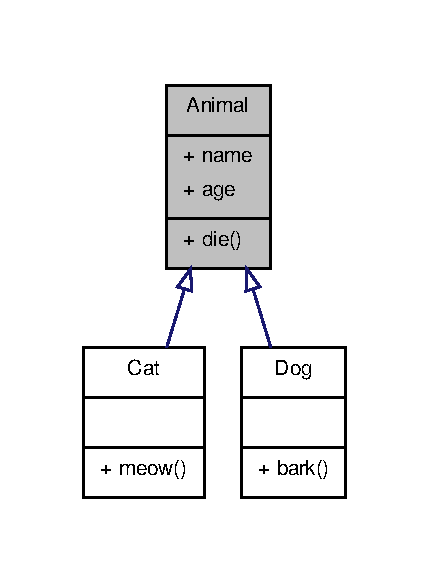
\includegraphics[width=206pt]{class_animal__inherit__graph}
\end{center}
\end{figure}


Collaboration diagram for Animal\-:
\nopagebreak
\begin{figure}[H]
\begin{center}
\leavevmode
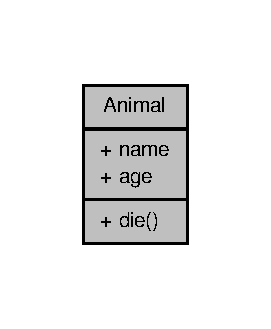
\includegraphics[width=130pt]{class_animal__coll__graph}
\end{center}
\end{figure}
\subsection*{Public Member Functions}
\begin{DoxyCompactItemize}
\item 
\hypertarget{class_animal_a557fe0d71dda75be2f8459ce0d7c2275}{void {\bfseries die} ()}\label{class_animal_a557fe0d71dda75be2f8459ce0d7c2275}

\end{DoxyCompactItemize}
\subsection*{Public Attributes}
\begin{DoxyCompactItemize}
\item 
\hypertarget{class_animal_a9cf3bfd9070daec7b3bbc87cbd958f35}{string {\bfseries name}}\label{class_animal_a9cf3bfd9070daec7b3bbc87cbd958f35}

\item 
\hypertarget{class_animal_a31e4a23bef9596927496de4eb6b9c721}{int {\bfseries age}}\label{class_animal_a31e4a23bef9596927496de4eb6b9c721}

\end{DoxyCompactItemize}


The documentation for this class was generated from the following file\-:\begin{DoxyCompactItemize}
\item 
test.\-cpp\end{DoxyCompactItemize}

\hypertarget{class_cat}{\section{Cat Class Reference}
\label{class_cat}\index{Cat@{Cat}}
}


Inheritance diagram for Cat\+:\nopagebreak
\begin{figure}[H]
\begin{center}
\leavevmode
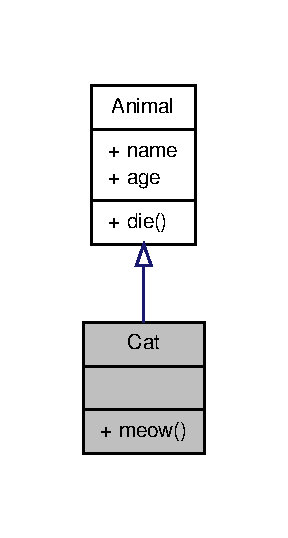
\includegraphics[width=138pt]{class_cat__inherit__graph}
\end{center}
\end{figure}


Collaboration diagram for Cat\+:\nopagebreak
\begin{figure}[H]
\begin{center}
\leavevmode
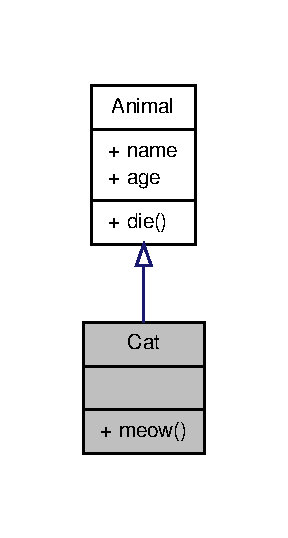
\includegraphics[width=138pt]{class_cat__coll__graph}
\end{center}
\end{figure}
\subsection*{Public Member Functions}
\begin{DoxyCompactItemize}
\item 
void \hyperlink{class_cat_aa770c672b7458b036d7384a6915d9367}{meow} ()
\end{DoxyCompactItemize}
\subsection*{Additional Inherited Members}


\subsection{Member Function Documentation}
\hypertarget{class_cat_aa770c672b7458b036d7384a6915d9367}{\index{Cat@{Cat}!meow@{meow}}
\index{meow@{meow}!Cat@{Cat}}
\subsubsection[{meow}]{\setlength{\rightskip}{0pt plus 5cm}void Cat\+::meow (
\begin{DoxyParamCaption}
{}
\end{DoxyParamCaption}
)}}\label{class_cat_aa770c672b7458b036d7384a6915d9367}


The documentation for this class was generated from the following file\+:\begin{DoxyCompactItemize}
\item 
\hyperlink{test_8cpp}{test.\+cpp}\end{DoxyCompactItemize}

\hypertarget{class_dog}{\section{Dog Class Reference}
\label{class_dog}\index{Dog@{Dog}}
}


Inheritance diagram for Dog\+:\nopagebreak
\begin{figure}[H]
\begin{center}
\leavevmode
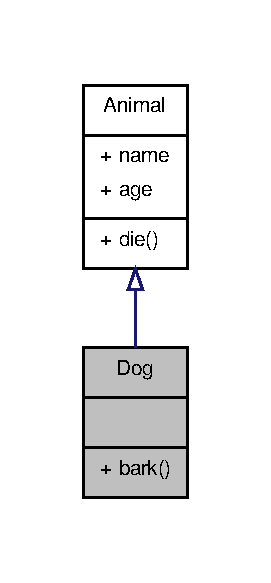
\includegraphics[width=130pt]{class_dog__inherit__graph}
\end{center}
\end{figure}


Collaboration diagram for Dog\+:\nopagebreak
\begin{figure}[H]
\begin{center}
\leavevmode
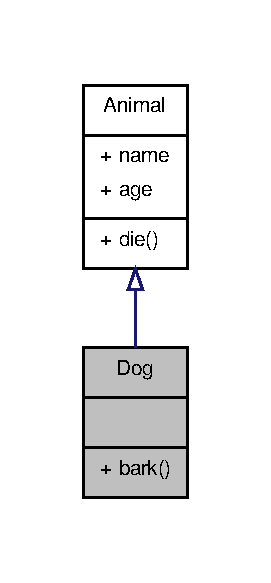
\includegraphics[width=130pt]{class_dog__coll__graph}
\end{center}
\end{figure}
\subsection*{Public Member Functions}
\begin{DoxyCompactItemize}
\item 
void \hyperlink{class_dog_ad3ab5661e3663948a486ff73049b1e1f}{bark} ()
\end{DoxyCompactItemize}
\subsection*{Additional Inherited Members}


\subsection{Member Function Documentation}
\hypertarget{class_dog_ad3ab5661e3663948a486ff73049b1e1f}{\index{Dog@{Dog}!bark@{bark}}
\index{bark@{bark}!Dog@{Dog}}
\subsubsection[{bark}]{\setlength{\rightskip}{0pt plus 5cm}void Dog\+::bark (
\begin{DoxyParamCaption}
{}
\end{DoxyParamCaption}
)}}\label{class_dog_ad3ab5661e3663948a486ff73049b1e1f}


The documentation for this class was generated from the following file\+:\begin{DoxyCompactItemize}
\item 
\hyperlink{test_8cpp}{test.\+cpp}\end{DoxyCompactItemize}

\hypertarget{classdoxygen__python_1_1_sample_class}{\section{doxygen\+\_\+python.\+Sample\+Class Class Reference}
\label{classdoxygen__python_1_1_sample_class}\index{doxygen\+\_\+python.\+Sample\+Class@{doxygen\+\_\+python.\+Sample\+Class}}
}


Inheritance diagram for doxygen\+\_\+python.\+Sample\+Class\+:\nopagebreak
\begin{figure}[H]
\begin{center}
\leavevmode
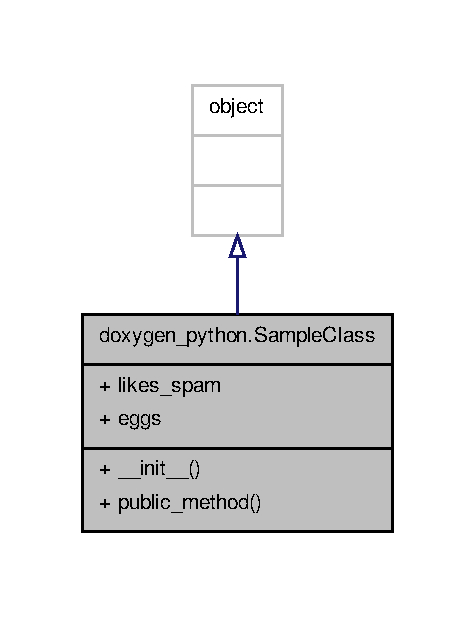
\includegraphics[width=228pt]{classdoxygen__python_1_1_sample_class__inherit__graph}
\end{center}
\end{figure}


Collaboration diagram for doxygen\+\_\+python.\+Sample\+Class\+:\nopagebreak
\begin{figure}[H]
\begin{center}
\leavevmode
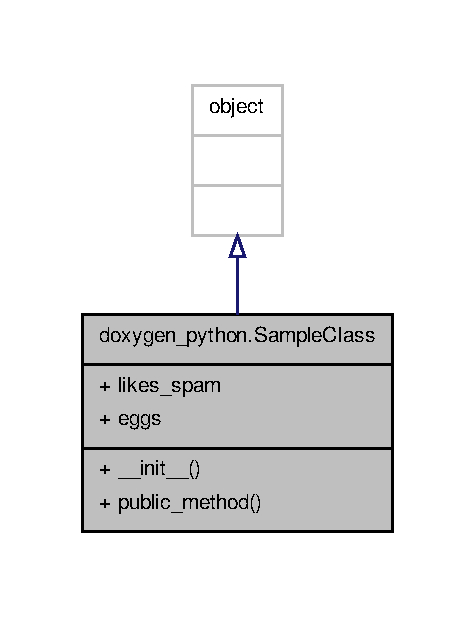
\includegraphics[width=228pt]{classdoxygen__python_1_1_sample_class__coll__graph}
\end{center}
\end{figure}
\subsection*{Public Member Functions}
\begin{DoxyCompactItemize}
\item 
def \hyperlink{classdoxygen__python_1_1_sample_class_a834388424360bc7f8812f12bcae9c6b0}{\+\_\+\+\_\+init\+\_\+\+\_\+}
\item 
def \hyperlink{classdoxygen__python_1_1_sample_class_a4f8ade12e6a2bea87688b62c6b381539}{public\+\_\+method}
\end{DoxyCompactItemize}
\subsection*{Public Attributes}
\begin{DoxyCompactItemize}
\item 
\hyperlink{classdoxygen__python_1_1_sample_class_aef079904f13e12bd0bdf168b469f0dd7}{likes\+\_\+spam}
\item 
\hyperlink{classdoxygen__python_1_1_sample_class_abbb2efa1b130ed66e847205b38d5ba5f}{eggs}
\end{DoxyCompactItemize}


\subsection{Detailed Description}
\begin{DoxyVerb}Summary of class here.

Longer class information....
Longer class information....

Attributes:
    likes_spam: A boolean indicating if we like SPAM or not.
    eggs: An integer count of the eggs we have laid.
\end{DoxyVerb}
 

\subsection{Constructor \& Destructor Documentation}
\hypertarget{classdoxygen__python_1_1_sample_class_a834388424360bc7f8812f12bcae9c6b0}{\index{doxygen\+\_\+python\+::\+Sample\+Class@{doxygen\+\_\+python\+::\+Sample\+Class}!\+\_\+\+\_\+init\+\_\+\+\_\+@{\+\_\+\+\_\+init\+\_\+\+\_\+}}
\index{\+\_\+\+\_\+init\+\_\+\+\_\+@{\+\_\+\+\_\+init\+\_\+\+\_\+}!doxygen\+\_\+python\+::\+Sample\+Class@{doxygen\+\_\+python\+::\+Sample\+Class}}
\subsubsection[{\+\_\+\+\_\+init\+\_\+\+\_\+}]{\setlength{\rightskip}{0pt plus 5cm}def doxygen\+\_\+python.\+Sample\+Class.\+\_\+\+\_\+init\+\_\+\+\_\+ (
\begin{DoxyParamCaption}
\item[{}]{self, }
\item[{}]{likes\+\_\+spam = {\ttfamily False}}
\end{DoxyParamCaption}
)}}\label{classdoxygen__python_1_1_sample_class_a834388424360bc7f8812f12bcae9c6b0}
\begin{DoxyVerb}Inits SampleClass with blah.\end{DoxyVerb}
 

\subsection{Member Function Documentation}
\hypertarget{classdoxygen__python_1_1_sample_class_a4f8ade12e6a2bea87688b62c6b381539}{\index{doxygen\+\_\+python\+::\+Sample\+Class@{doxygen\+\_\+python\+::\+Sample\+Class}!public\+\_\+method@{public\+\_\+method}}
\index{public\+\_\+method@{public\+\_\+method}!doxygen\+\_\+python\+::\+Sample\+Class@{doxygen\+\_\+python\+::\+Sample\+Class}}
\subsubsection[{public\+\_\+method}]{\setlength{\rightskip}{0pt plus 5cm}def doxygen\+\_\+python.\+Sample\+Class.\+public\+\_\+method (
\begin{DoxyParamCaption}
\item[{}]{self}
\end{DoxyParamCaption}
)}}\label{classdoxygen__python_1_1_sample_class_a4f8ade12e6a2bea87688b62c6b381539}
\begin{DoxyVerb}Performs operation blah.\end{DoxyVerb}
 

\subsection{Member Data Documentation}
\hypertarget{classdoxygen__python_1_1_sample_class_abbb2efa1b130ed66e847205b38d5ba5f}{\index{doxygen\+\_\+python\+::\+Sample\+Class@{doxygen\+\_\+python\+::\+Sample\+Class}!eggs@{eggs}}
\index{eggs@{eggs}!doxygen\+\_\+python\+::\+Sample\+Class@{doxygen\+\_\+python\+::\+Sample\+Class}}
\subsubsection[{eggs}]{\setlength{\rightskip}{0pt plus 5cm}doxygen\+\_\+python.\+Sample\+Class.\+eggs}}\label{classdoxygen__python_1_1_sample_class_abbb2efa1b130ed66e847205b38d5ba5f}
\hypertarget{classdoxygen__python_1_1_sample_class_aef079904f13e12bd0bdf168b469f0dd7}{\index{doxygen\+\_\+python\+::\+Sample\+Class@{doxygen\+\_\+python\+::\+Sample\+Class}!likes\+\_\+spam@{likes\+\_\+spam}}
\index{likes\+\_\+spam@{likes\+\_\+spam}!doxygen\+\_\+python\+::\+Sample\+Class@{doxygen\+\_\+python\+::\+Sample\+Class}}
\subsubsection[{likes\+\_\+spam}]{\setlength{\rightskip}{0pt plus 5cm}doxygen\+\_\+python.\+Sample\+Class.\+likes\+\_\+spam}}\label{classdoxygen__python_1_1_sample_class_aef079904f13e12bd0bdf168b469f0dd7}


The documentation for this class was generated from the following file\+:\begin{DoxyCompactItemize}
\item 
\hyperlink{doxygen__python_8py}{doxygen\+\_\+python.\+py}\end{DoxyCompactItemize}

\hypertarget{classtest_1_1_staterobot}{\section{test.\-Staterobot Class Reference}
\label{classtest_1_1_staterobot}\index{test.\-Staterobot@{test.\-Staterobot}}
}


Inheritance diagram for test.\-Staterobot\-:
\nopagebreak
\begin{figure}[H]
\begin{center}
\leavevmode
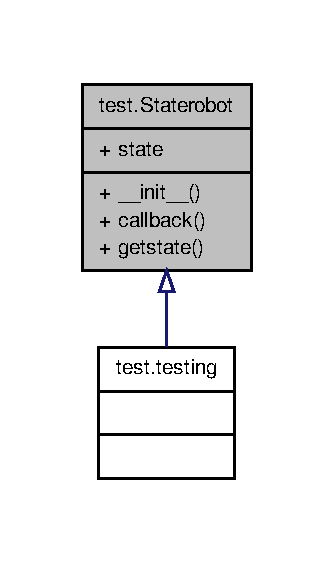
\includegraphics[width=160pt]{classtest_1_1_staterobot__inherit__graph}
\end{center}
\end{figure}


Collaboration diagram for test.\-Staterobot\-:
\nopagebreak
\begin{figure}[H]
\begin{center}
\leavevmode
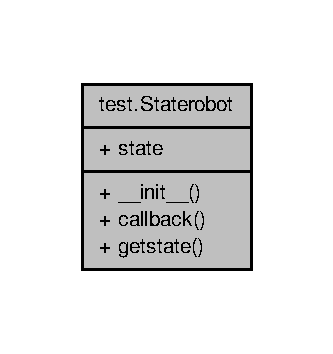
\includegraphics[width=160pt]{classtest_1_1_staterobot__coll__graph}
\end{center}
\end{figure}
\subsection*{Public Member Functions}
\begin{DoxyCompactItemize}
\item 
\hypertarget{classtest_1_1_staterobot_a825aa6cfc4a937fae93b18eb22d5049d}{def {\bfseries \-\_\-\-\_\-init\-\_\-\-\_\-}}\label{classtest_1_1_staterobot_a825aa6cfc4a937fae93b18eb22d5049d}

\item 
\hypertarget{classtest_1_1_staterobot_a2c8f2fc540f84bfc18477fdde6510bfa}{def {\bfseries callback}}\label{classtest_1_1_staterobot_a2c8f2fc540f84bfc18477fdde6510bfa}

\item 
\hypertarget{classtest_1_1_staterobot_a5663f3bcd6262303e19c4735396cbef2}{def {\bfseries getstate}}\label{classtest_1_1_staterobot_a5663f3bcd6262303e19c4735396cbef2}

\end{DoxyCompactItemize}
\subsection*{Public Attributes}
\begin{DoxyCompactItemize}
\item 
\hypertarget{classtest_1_1_staterobot_a6ac3890142e62ba6a4e96f3090fa9b38}{{\bfseries state}}\label{classtest_1_1_staterobot_a6ac3890142e62ba6a4e96f3090fa9b38}

\end{DoxyCompactItemize}


The documentation for this class was generated from the following file\-:\begin{DoxyCompactItemize}
\item 
test.\-py\end{DoxyCompactItemize}

\hypertarget{classtest_1_1testing}{\section{test.\-testing Class Reference}
\label{classtest_1_1testing}\index{test.\-testing@{test.\-testing}}
}


Inheritance diagram for test.\-testing\-:
\nopagebreak
\begin{figure}[H]
\begin{center}
\leavevmode
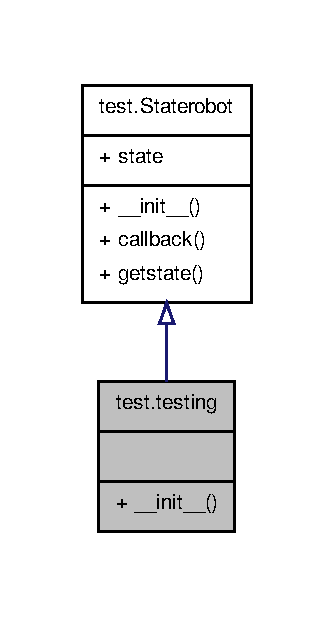
\includegraphics[width=160pt]{classtest_1_1testing__inherit__graph}
\end{center}
\end{figure}


Collaboration diagram for test.\-testing\-:
\nopagebreak
\begin{figure}[H]
\begin{center}
\leavevmode
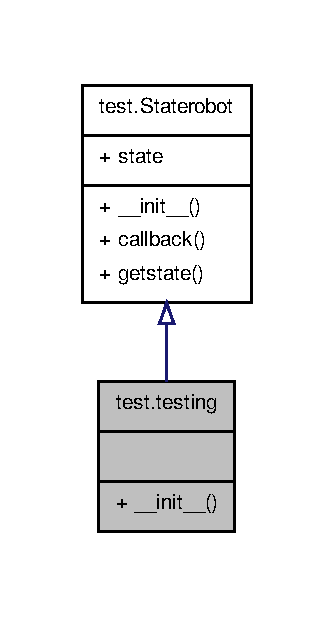
\includegraphics[width=160pt]{classtest_1_1testing__coll__graph}
\end{center}
\end{figure}
\subsection*{Additional Inherited Members}


The documentation for this class was generated from the following file\-:\begin{DoxyCompactItemize}
\item 
test.\-py\end{DoxyCompactItemize}

\chapter{File Documentation}
\hypertarget{doxygen__python_8py}{\section{doxygen\+\_\+python.\+py File Reference}
\label{doxygen__python_8py}\index{doxygen\+\_\+python.\+py@{doxygen\+\_\+python.\+py}}
}
\subsection*{Classes}
\begin{DoxyCompactItemize}
\item 
class \hyperlink{classdoxygen__python_1_1_sample_class}{doxygen\+\_\+python.\+Sample\+Class}
\end{DoxyCompactItemize}
\subsection*{Namespaces}
\begin{DoxyCompactItemize}
\item 
 \hyperlink{namespacedoxygen__python}{doxygen\+\_\+python}
\end{DoxyCompactItemize}
\subsection*{Functions}
\begin{DoxyCompactItemize}
\item 
def \hyperlink{namespacedoxygen__python_a5c92544fbb20cd4315a7f365b7280bd1}{doxygen\+\_\+python.\+fetch\+\_\+bigtable\+\_\+rows}
\end{DoxyCompactItemize}
\subsection*{Variables}
\begin{DoxyCompactItemize}
\item 
\hyperlink{namespacedoxygen__python_a2955b270349986df67d20bc386a54b90}{doxygen\+\_\+python.\+i} = None
\end{DoxyCompactItemize}

\hypertarget{test_8cpp}{\section{test.\+cpp File Reference}
\label{test_8cpp}\index{test.\+cpp@{test.\+cpp}}
}
\subsection*{Classes}
\begin{DoxyCompactItemize}
\item 
class \hyperlink{class_animal}{Animal}
\item 
class \hyperlink{class_dog}{Dog}
\item 
class \hyperlink{class_cat}{Cat}
\end{DoxyCompactItemize}

\hypertarget{test_8py}{\section{test.\+py File Reference}
\label{test_8py}\index{test.\+py@{test.\+py}}
}
\subsection*{Classes}
\begin{DoxyCompactItemize}
\item 
class \hyperlink{classtest_1_1_staterobot}{test.\+Staterobot}
\item 
class \hyperlink{classtest_1_1testing}{test.\+testing}
\end{DoxyCompactItemize}
\subsection*{Namespaces}
\begin{DoxyCompactItemize}
\item 
 \hyperlink{namespacetest}{test}
\end{DoxyCompactItemize}
\subsection*{Variables}
\begin{DoxyCompactItemize}
\item 
tuple \hyperlink{namespacetest_adf753579d10a80fa8ab7e3763b1089be}{test.\+obj} = Staterobot('/ground\+\_\+truth/state')
\end{DoxyCompactItemize}

%--- End generated contents ---

% Index
\newpage
\phantomsection
\addcontentsline{toc}{chapter}{Index}
\printindex

\end{document}
